\documentclass[final]{beamer}

\usepackage[
  orientation=portrait,
  size=custom,
  width=61,      % 24 inches = 60.96 cm
  height=91.44,  % 36 inches = 91.44 cm
  scale=1.0
]{beamerposter}

\usepackage{graphicx}
\usepackage{booktabs}
\usepackage{colortbl}
\usepackage{xcolor}
\usepackage{amsmath}
\usepackage{array}
\usepackage{calc}
\usepackage[T1]{fontenc}
\usepackage{lmodern}

\graphicspath{{figures/}}

% ── Method identity colors ──────────────────────────────────────────────────
\definecolor{ilpred}{HTML}{E53935}
\definecolor{pbgreen}{HTML}{43A047}
\definecolor{ppoblue}{HTML}{1E88E5}
\definecolor{scimlorg}{HTML}{FB8C00}

% ── Table cell colors ───────────────────────────────────────────────────────
\definecolor{cellgreen}{HTML}{C8E6C9}
\definecolor{cellred}{HTML}{FFCDD2}
\definecolor{cellamber}{HTML}{FFE082}
\definecolor{cellgray}{HTML}{F0F0F0}

% ── Beamer theme ─────────────────────────────────────────────────────────────
\usetheme{default}
\usecolortheme{default}
\setbeamertemplate{navigation symbols}{}
\setbeamerfont{block title}{size=\large,series=\bfseries}
\setbeamerfont{block body}{size=\normalsize}
\setbeamercolor{structure}{fg=black}

% ── Per-method colored block environments ────────────────────────────────────
\newenvironment{ilpblock}[1]{%
  \setbeamercolor{block title}{fg=white,bg=ilpred}%
  \setbeamercolor{block body}{fg=black,bg=ilpred!8}%
  \begin{block}{#1}}{\end{block}}

\newenvironment{pbblock}[1]{%
  \setbeamercolor{block title}{fg=white,bg=pbgreen}%
  \setbeamercolor{block body}{fg=black,bg=pbgreen!8}%
  \begin{block}{#1}}{\end{block}}

\newenvironment{ppoblock}[1]{%
  \setbeamercolor{block title}{fg=white,bg=ppoblue}%
  \setbeamercolor{block body}{fg=black,bg=ppoblue!8}%
  \begin{block}{#1}}{\end{block}}

\newenvironment{scimlblock}[1]{%
  \setbeamercolor{block title}{fg=white,bg=scimlorg}%
  \setbeamercolor{block body}{fg=black,bg=scimlorg!8}%
  \begin{block}{#1}}{\end{block}}

% ── Convenience: gray section block ──────────────────────────────────────────
\newenvironment{grayblock}[1]{%
  \setbeamercolor{block title}{fg=white,bg=gray!70}%
  \setbeamercolor{block body}{fg=black,bg=gray!6}%
  \begin{block}{#1}}{\end{block}}

% ── Reduce default block padding ─────────────────────────────────────────────
\setbeamertemplate{block begin}{
  \vskip0.15cm
  \begin{beamercolorbox}[rounded=true,shadow=false,leftskip=0.4cm,rightskip=0.4cm,dp=0.2cm]{block title}
    \usebeamerfont{block title}\insertblocktitle
  \end{beamercolorbox}
  \nointerlineskip
  \begin{beamercolorbox}[rounded=true,shadow=false,leftskip=0.4cm,rightskip=0.4cm,vmode]{block body}
    \vskip0.2cm
}
\setbeamertemplate{block end}{
    \vskip0.2cm
  \end{beamercolorbox}
  \vskip0.1cm
}

% ── Font sizes for poster scale ───────────────────────────────────────────────
% beamerposter scale=1.0 on a 61x91 cm canvas maps \normalsize ≈ 20pt,
% \large ≈ 24pt, \Large ≈ 28pt, \LARGE ≈ 34pt, \huge ≈ 40pt, \Huge ≈ 48pt.

\begin{document}
\begin{frame}[t]

% ════════════════════════════════════════════════════════════════════════════
% TITLE BANNER
% ════════════════════════════════════════════════════════════════════════════
\begin{columns}[t]
  \begin{column}{\textwidth}
    \vspace{0.3cm}
    {\bfseries\LARGE Four Methods, One Problem: The No-Three-In-Line Problem\par}
    \vspace{0.2cm}
    {\large
      Pranav Ramanathan$^{1}$,\;
      Thomas Prellberg$^{1}$,\;
      Prathamesh Dinesh Joshi$^{2}$,\;
      Raj Abhijit Dandekar$^{2}$,\;
      Rajat Dandekar$^{2}$,\;
      Sreedath Panat$^{2}$\par}
    \vspace{0.1cm}
    {\normalsize
      $^{1}$School of Mathematical Sciences, Queen Mary University of London\quad
      $^{2}$Vizuara AI Labs\par}
    \vspace{0.15cm}
    {\large\itshape ILP certifies.\enspace PatternBoost learns.\enspace PPO places.\enspace SciML reaches.\par}
    \vspace{0.2cm}
    \begin{columns}[c]
      \begin{column}{0.73\textwidth}
        \begin{itemize}\setlength\itemsep{0.1em}
          \item \textbf{ILP} certifies provably optimal solutions to $n=19$ — no ML method matches this guarantee
          \item \textbf{SciML} (gradient flow, Apple M2 Metal, no symmetry pruning) solves $n=18$ in 9/10 runs
          \item \textbf{Continuous relaxation} extends ML reach well beyond the discrete-search ceilings of transformer and RL methods
        \end{itemize}
      \end{column}
      \begin{column}{0.25\textwidth}
        \centering
        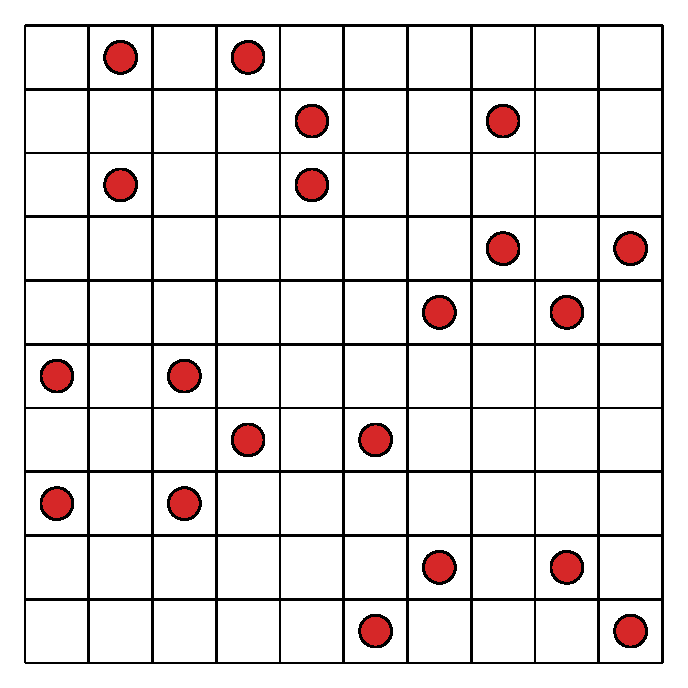
\includegraphics[height=7cm,keepaspectratio]{no_three_in_line_n10.pdf}\\[2pt]
        {\small Optimal $10{\times}10$ solution (20 pts)}
      \end{column}
    \end{columns}
    \vspace{0.2cm}
    \hrule height 1.2pt
    \vspace{0.2cm}
  \end{column}
\end{columns}

% ════════════════════════════════════════════════════════════════════════════
% PROBLEM
% ════════════════════════════════════════════════════════════════════════════
\begin{columns}[t]
  \begin{column}{\textwidth}
    \begin{grayblock}{1.\enspace The No-Three-In-Line Problem}
      Place the \textbf{maximum} number of points on an $n\times n$ integer grid such that
      \textbf{no three points are collinear}.
      Trivial upper bound: $2n$ (pigeonhole).
      Best proven lower bound: $\approx1.5n$ (Hall et al.\ 1975).
      Exact optimal known to $n\approx19$ with symmetry pruning; $n\ge20$ open.
    \end{grayblock}
    \vspace{0.15cm}
  \end{column}
\end{columns}

% ════════════════════════════════════════════════════════════════════════════
% METHOD PANELS  (2 × 2)
% ════════════════════════════════════════════════════════════════════════════
\begin{columns}[t,totalwidth=\textwidth]

  % ── LEFT COLUMN ───────────────────────────────────────────────────────────
  \begin{column}{0.492\textwidth}

    \begin{ilpblock}{2a.\enspace Integer Linear Programming (ILP)}
      \begin{itemize}\setlength\itemsep{0.05em}
        \item Collinearity encoded as linear constraints; solved by Gurobi branch-and-bound
        \item \textbf{Certifiably optimal} at every $n$ tested ($n\le19$)
        \item Exponential worst-case scaling; symmetry pruning essential for $n\ge15$
      \end{itemize}
      \vspace{0.2cm}
      \centering
      \large\bfseries\color{ilpred}Certified optimal to $n=19$
    \end{ilpblock}

    \vspace{0.2cm}

    \begin{ppoblock}{2c.\enspace Proximal Policy Optimisation (PPO)}
      \begin{itemize}\setlength\itemsep{0.05em}
        \item RL agent learns a point-placement policy on the $n\times n$ grid
        \item Perfect solutions at $n=10$; one collinearity violation at $n=11$ (shown right $\rightarrow$)
        \item Discrete action space scales as $n^2$ — key scalability bottleneck
      \end{itemize}
      \vspace{0.15cm}
      \begin{columns}[c]
        \begin{column}{0.475\linewidth}
          \centering
          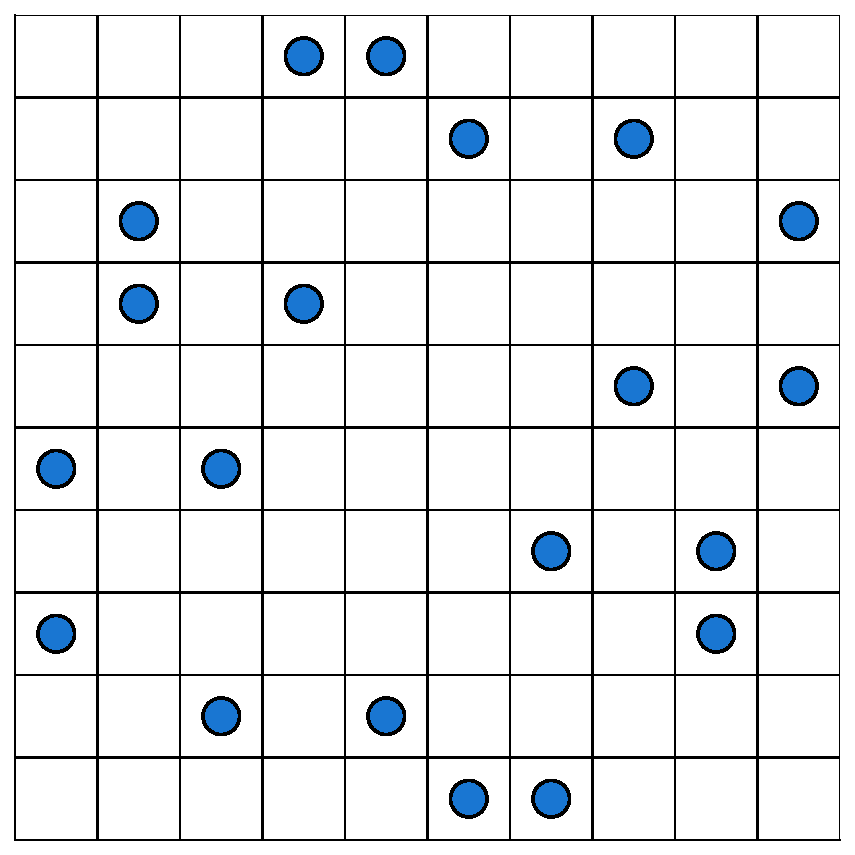
\includegraphics[height=7cm,keepaspectratio]{best_model_final_state_n10.pdf}\\[2pt]
          {\small $n=10$:\enspace\textbf{20 pts, 0 violations}}
        \end{column}
        \begin{column}{0.475\linewidth}
          \centering
          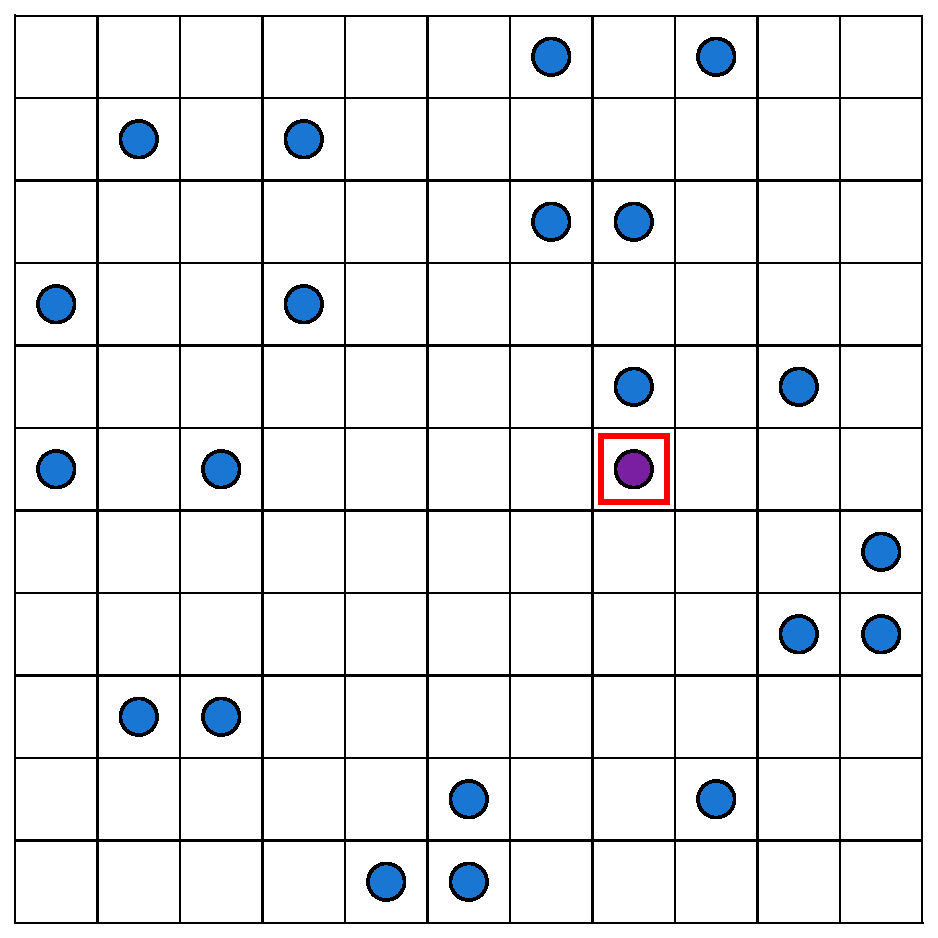
\includegraphics[height=7cm,keepaspectratio]{best_model_final_state_n11.pdf}\\[2pt]
          {\small $n=11$:\enspace\textbf{22 pts, 1 violation} {\color{red}$\leftarrow$}}
        \end{column}
      \end{columns}
      \vspace{0.15cm}
      \centering
      \large\bfseries\color{ppoblue}Hits constraint wall at $n=11$
    \end{ppoblock}

  \end{column}

  % ── GUTTER ────────────────────────────────────────────────────────────────
  \begin{column}{0.016\textwidth}\end{column}

  % ── RIGHT COLUMN ──────────────────────────────────────────────────────────
  \begin{column}{0.492\textwidth}

    \begin{pbblock}{2b.\enspace PatternBoost (Transformer)}
      \begin{itemize}\setlength\itemsep{0.05em}
        \item Transformer trained on known solutions learns N3L geometric patterns
        \item Iterative boosting: weak candidates regenerated; matches optimal to $n=14$
        \item Finds 29/30 points at $n=15$ (optimal is 30)
      \end{itemize}
      \vspace{0.15cm}
      \begin{columns}[c]
        \begin{column}{0.475\linewidth}
          \centering
          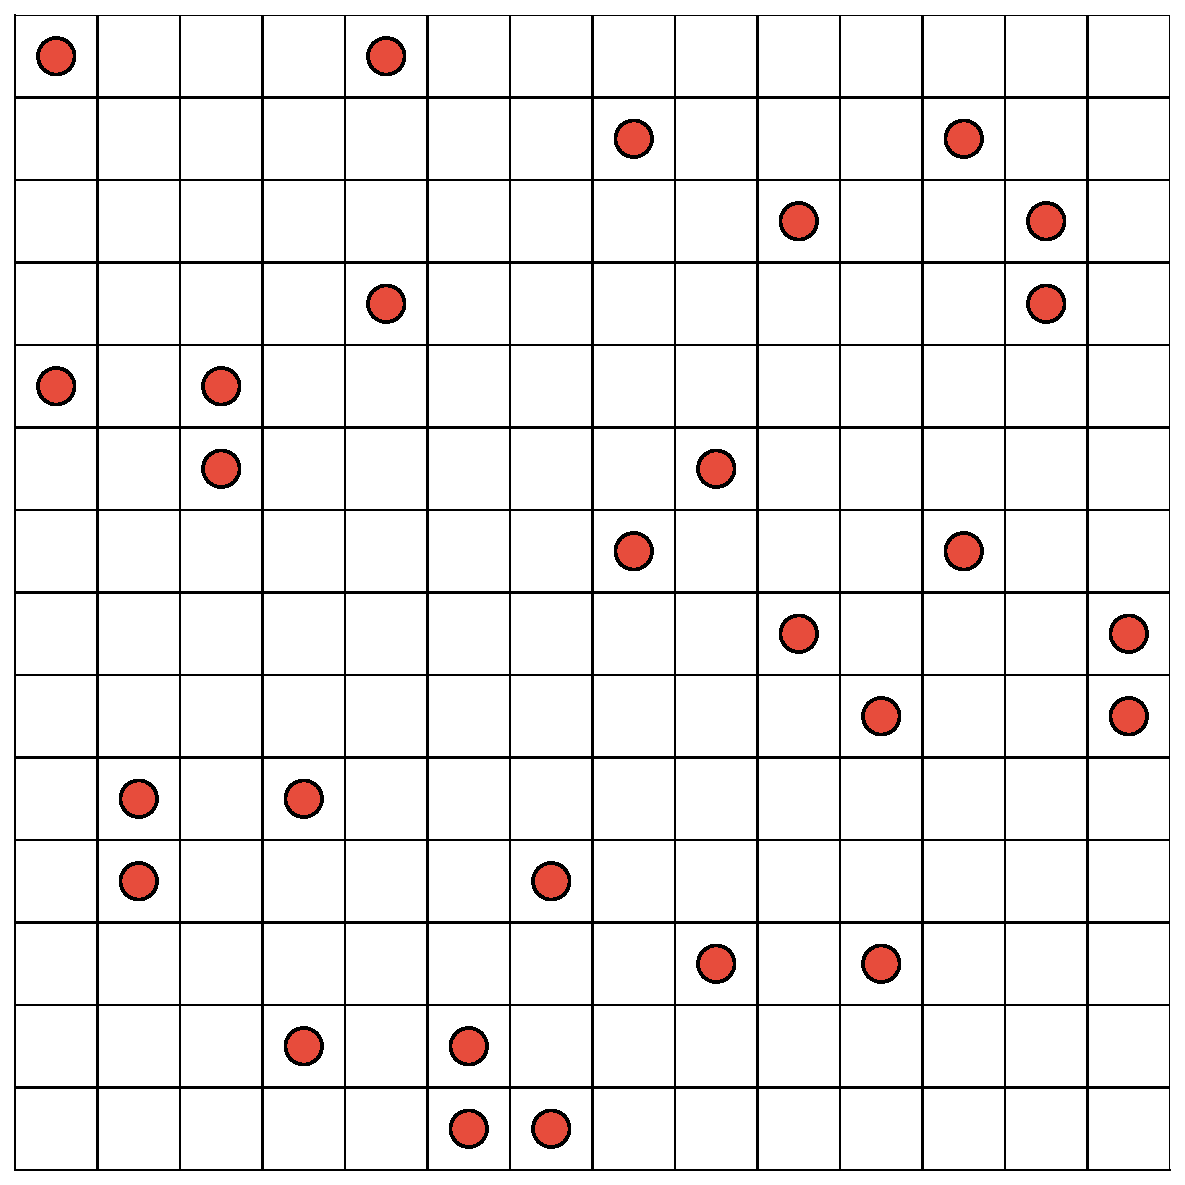
\includegraphics[height=7cm,keepaspectratio]{PatternBoost_n14.pdf}\\[2pt]
          {\small $n=14$:\enspace\textbf{28 pts} (optimal)}
        \end{column}
        \begin{column}{0.475\linewidth}
          \centering
          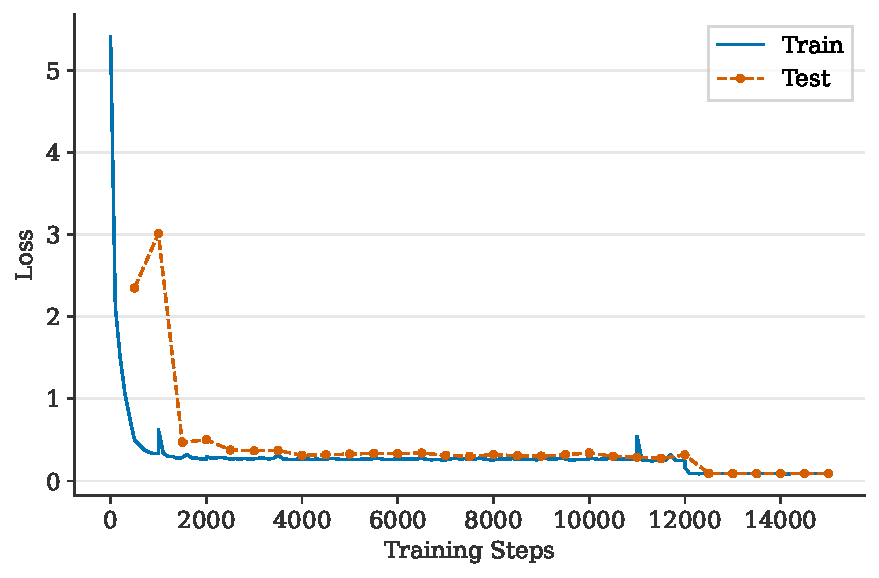
\includegraphics[height=7cm,keepaspectratio]{loss_plot.pdf}\\[2pt]
          {\small Training loss}
        \end{column}
      \end{columns}
      \vspace{0.15cm}
      \centering
      \large\bfseries\color{pbgreen}Optimal to $n=14$;\enspace 29/30 at $n=15$
    \end{pbblock}

    \vspace{0.2cm}

    \begin{scimlblock}{2d.\enspace Scientific Machine Learning (SciML)}
      \begin{itemize}\setlength\itemsep{0.05em}
        \item Recasts N3L as continuous energy minimisation solved by gradient flow:
          $E = \alpha E_{\text{coll}} + E_{\text{count}} + \mu E_{\text{bin}}$
        \item Custom Metal GPU kernel (Julia, Apple M2); no symmetry pruning
        \item Non-monotonic reliability: $n=17$ fails (0/10); $n=18$ succeeds (9/10)
      \end{itemize}
      \vspace{0.1cm}
      \begin{columns}[c]
        \begin{column}{0.515\linewidth}
          \centering
          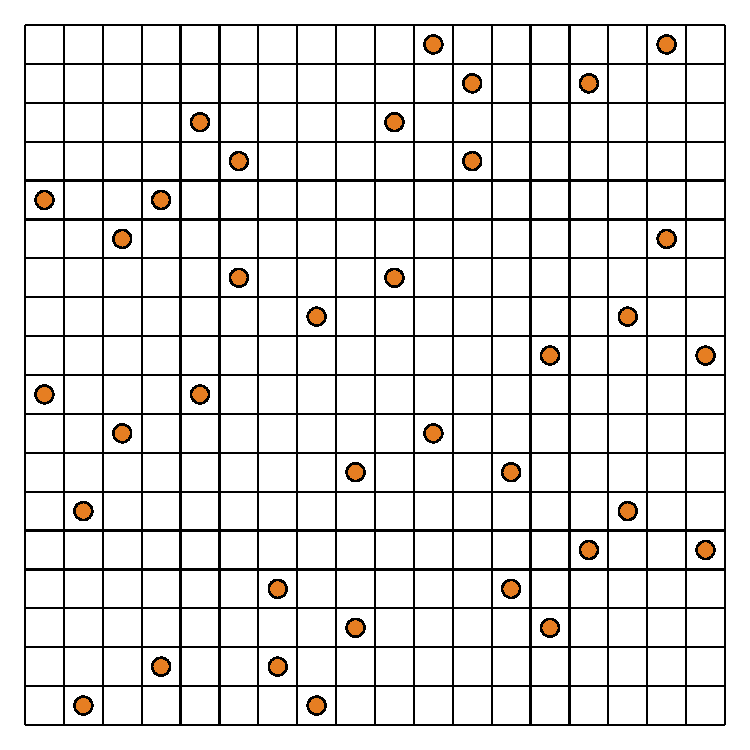
\includegraphics[height=8cm,keepaspectratio]{sciml_solution_n18.pdf}\\[2pt]
          {\small $n=18$:\enspace\textbf{36 pts, 0 violations} (9/10 runs)}
        \end{column}
        \begin{column}{0.455\linewidth}
          \centering
          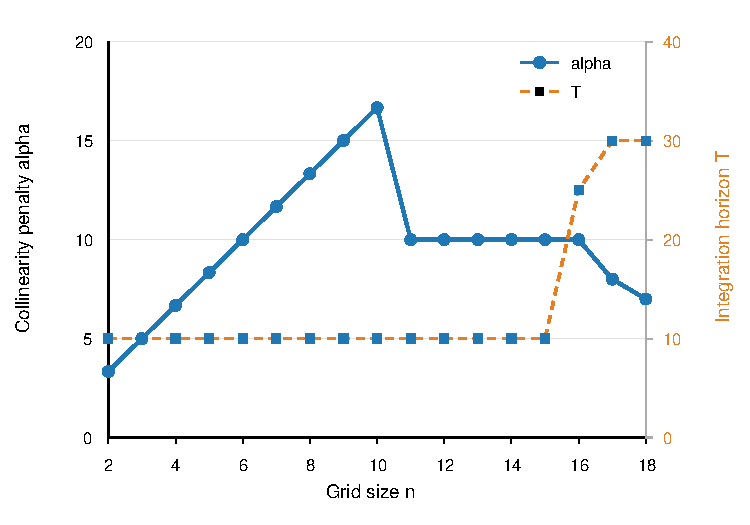
\includegraphics[height=8cm,keepaspectratio]{sciml_alpha_scaling.pdf}\\[2pt]
          {\small $\alpha$, $T$ schedule across $n$}
        \end{column}
      \end{columns}
      \vspace{0.15cm}
      \centering
      \large\bfseries\color{scimlorg}Reaches $n=18$ without symmetry pruning
    \end{scimlblock}

  \end{column}
\end{columns}

\vspace{0.2cm}

% ════════════════════════════════════════════════════════════════════════════
% RESULTS TABLE
% ════════════════════════════════════════════════════════════════════════════
\begin{columns}[t]
  \begin{column}{\textwidth}
    \begin{grayblock}{3.\enspace Results — Maximum Points Found ($\text{optimal} = 2n$)}
      \centering
      \renewcommand{\arraystretch}{1.15}
      \setlength{\tabcolsep}{5pt}
      \begin{tabular}{c|
          >{\centering}p{2.6cm}|
          >{\centering}p{3.4cm}|
          >{\centering}p{2.6cm}|
          >{\centering\arraybackslash}p{3.6cm}}
        \toprule
        \textbf{$n$} &
        \textbf{\color{ilpred}ILP} &
        \shortstack{\textbf{\color{pbgreen}Pattern-}\\\textbf{\color{pbgreen}Boost}} &
        \textbf{\color{ppoblue}PPO} &
        \shortstack{\textbf{\color{scimlorg}SciML}\\{\small(10 runs)}} \\
        \midrule
        10 & \cellcolor{cellgreen}20 & \cellcolor{cellgreen}20 & \cellcolor{cellgreen}20 & \cellcolor{cellgreen}20\enspace{\small(10/10)} \\
        11 & \cellcolor{cellgreen}22 & \cellcolor{cellgreen}22 & \cellcolor{cellred}22$^{\star}$ & \cellcolor{cellgreen}22\enspace{\small(7/10)} \\
        12 & \cellcolor{cellgreen}24 & \cellcolor{cellgreen}24 & \cellcolor{cellgray}-- & \cellcolor{cellgreen}24\enspace{\small(10/10)} \\
        13 & \cellcolor{cellgreen}26 & \cellcolor{cellgreen}26 & \cellcolor{cellgray}-- & \cellcolor{cellgreen}26\enspace{\small(8/10)} \\
        14 & \cellcolor{cellgreen}28 & \cellcolor{cellgreen}28 & \cellcolor{cellgray}-- & \cellcolor{cellgreen}28\enspace{\small(4/10)} \\
        15 & \cellcolor{cellgreen}30 & \cellcolor{cellamber}29 & \cellcolor{cellgray}-- & \cellcolor{cellgreen}30\enspace{\small(8/10)} \\
        16 & \cellcolor{cellgreen}32 & \cellcolor{cellgray}-- & \cellcolor{cellgray}-- & \cellcolor{cellgreen}32\enspace{\small(8/10)} \\
        17 & \cellcolor{cellgreen}34 & \cellcolor{cellgray}-- & \cellcolor{cellgray}-- & \cellcolor{cellred}0/10$^{\dagger}$ \\
        18 & \cellcolor{cellgreen}36 & \cellcolor{cellgray}-- & \cellcolor{cellgray}-- & \cellcolor{cellgreen}36\enspace{\small(9/10)} \\
        19 & \cellcolor{cellgreen}38 & \cellcolor{cellgray}-- & \cellcolor{cellgray}-- & \cellcolor{cellred}0/10 \\
        \bottomrule
      \end{tabular}

      \vspace{0.15cm}
      {\small
        \colorbox{cellgreen}{\phantom{X}}~Optimal ($2n$)\enspace
        \colorbox{cellamber}{\phantom{X}}~Sub-optimal\enspace
        \colorbox{cellred}{\phantom{X}}~Violation/failure\enspace
        \colorbox{cellgray}{\phantom{X}}~Not tested\par}
      \vspace{0.1cm}
      {\footnotesize
        $^{\star}$PPO $n=11$: 22 pts but 1 collinearity violation.\enspace
        $^{\dagger}$SciML $n=17$: 0/10 standard seeds; optimal for one isolated seed only.\par}
    \end{grayblock}
  \end{column}
\end{columns}

\vspace{0.2cm}

% ════════════════════════════════════════════════════════════════════════════
% TAKEAWAYS + QR
% ════════════════════════════════════════════════════════════════════════════
\begin{columns}[t]
  \begin{column}{0.71\textwidth}
    \setbeamercolor{block title}{fg=white,bg=black!78}
    \setbeamercolor{block body}{fg=black,bg=black!5}
    \begin{block}{4.\enspace Takeaways}
      \begin{itemize}\setlength\itemsep{0.1em}
        \item \textbf{Continuous relaxation is the key advance:} SciML reaches $n=18$ without
          symmetry pruning — beyond any prior ML solver for this problem
        \item \textbf{Exact guarantees still require ILP:} no learning-based method certifies optimality;
          the two paradigms are complementary, not competing
        \item \textbf{Non-monotonicity is informative:} $n=17$ failure despite $n=18$ success
          suggests energy-landscape sensitivity, not purely grid-size scaling
        \item \textbf{Future:} ILP+SciML warm-starting; extend to $n\ge20$; investigate $n=17$ failure
      \end{itemize}
    \end{block}
  \end{column}
  \begin{column}{0.015\textwidth}\end{column}
  \begin{column}{0.275\textwidth}
    \setbeamercolor{block title}{fg=white,bg=gray!60}
    \setbeamercolor{block body}{fg=black,bg=gray!6}
    \begin{block}{Paper \& Code}
      \centering
      \vspace{0.2cm}
      % ── Replace fbox with \includegraphics{qr_arxiv.png} once you have the URL ──
      \fbox{\parbox{5.5cm}{\centering\vspace{1.2cm}
        {\large QR CODE}\\[4pt]
        {\small add arXiv URL here}
        \vspace{1.2cm}}}
      \vspace{0.2cm}\\
      {\small ICML 2026 · AI for Math Workshop}\\[3pt]
      {\small \texttt{p.ramanathan@se23.qmul.ac.uk}}
    \end{block}
  \end{column}
\end{columns}

\vspace{0.15cm}

\end{frame}
\end{document}
